% Options for packages loaded elsewhere
\PassOptionsToPackage{unicode}{hyperref}
\PassOptionsToPackage{hyphens}{url}
\PassOptionsToPackage{dvipsnames,svgnames,x11names}{xcolor}
%
\documentclass[
]{report}

\usepackage{amsmath,amssymb}
\usepackage{iftex}
\ifPDFTeX
  \usepackage[T1]{fontenc}
  \usepackage[utf8]{inputenc}
  \usepackage{textcomp} % provide euro and other symbols
\else % if luatex or xetex
  \usepackage{unicode-math}
  \defaultfontfeatures{Scale=MatchLowercase}
  \defaultfontfeatures[\rmfamily]{Ligatures=TeX,Scale=1}
\fi
\usepackage{lmodern}
\ifPDFTeX\else  
    % xetex/luatex font selection
\fi
% Use upquote if available, for straight quotes in verbatim environments
\IfFileExists{upquote.sty}{\usepackage{upquote}}{}
\IfFileExists{microtype.sty}{% use microtype if available
  \usepackage[]{microtype}
  \UseMicrotypeSet[protrusion]{basicmath} % disable protrusion for tt fonts
}{}
\makeatletter
\@ifundefined{KOMAClassName}{% if non-KOMA class
  \IfFileExists{parskip.sty}{%
    \usepackage{parskip}
  }{% else
    \setlength{\parindent}{0pt}
    \setlength{\parskip}{6pt plus 2pt minus 1pt}}
}{% if KOMA class
  \KOMAoptions{parskip=half}}
\makeatother
\usepackage{xcolor}
\setlength{\emergencystretch}{3em} % prevent overfull lines
\setcounter{secnumdepth}{-\maxdimen} % remove section numbering
% Make \paragraph and \subparagraph free-standing
\ifx\paragraph\undefined\else
  \let\oldparagraph\paragraph
  \renewcommand{\paragraph}[1]{\oldparagraph{#1}\mbox{}}
\fi
\ifx\subparagraph\undefined\else
  \let\oldsubparagraph\subparagraph
  \renewcommand{\subparagraph}[1]{\oldsubparagraph{#1}\mbox{}}
\fi


\providecommand{\tightlist}{%
  \setlength{\itemsep}{0pt}\setlength{\parskip}{0pt}}\usepackage{longtable,booktabs,array}
\usepackage{calc} % for calculating minipage widths
% Correct order of tables after \paragraph or \subparagraph
\usepackage{etoolbox}
\makeatletter
\patchcmd\longtable{\par}{\if@noskipsec\mbox{}\fi\par}{}{}
\makeatother
% Allow footnotes in longtable head/foot
\IfFileExists{footnotehyper.sty}{\usepackage{footnotehyper}}{\usepackage{footnote}}
\makesavenoteenv{longtable}
\usepackage{graphicx}
\makeatletter
\def\maxwidth{\ifdim\Gin@nat@width>\linewidth\linewidth\else\Gin@nat@width\fi}
\def\maxheight{\ifdim\Gin@nat@height>\textheight\textheight\else\Gin@nat@height\fi}
\makeatother
% Scale images if necessary, so that they will not overflow the page
% margins by default, and it is still possible to overwrite the defaults
% using explicit options in \includegraphics[width, height, ...]{}
\setkeys{Gin}{width=\maxwidth,height=\maxheight,keepaspectratio}
% Set default figure placement to htbp
\makeatletter
\def\fps@figure{htbp}
\makeatother

\usepackage{booktabs}
\usepackage{amsthm}
\usepackage{placeins}
\makeatletter
\def\thm@space@setup{%
  \thm@preskip=8pt plus 2pt minus 4pt
  \thm@postskip=\thm@preskip
}
\makeatother
\usepackage{adjustbox}
\usepackage{awesomebox}
\usepackage{color}
\usepackage{framed}
\setlength{\fboxsep}{.8em}
\usepackage[most]{tcolorbox}
\usepackage{blindtext}
\usepackage{amsmath}
\usepackage{amssymb}
\usepackage{bm}
\usepackage[finnish]{babel}
\usepackage{graphicx}
\usepackage{placeins}
\usepackage{overpic}
\usepackage{lmodern}
\usepackage{epsfig}
\usepackage{placeins}
\usepackage{xstring}     % Used for \IfEqCase


\definecolor{myboxcolor}{named}{blue} % Default box color

\definecolor{my-purple}{RGB}{204,180,225}
\newtcolorbox{defblock}[1]{%
    breakable,
    enhanced,
    coltext=black,
    colback=my-purple,      % Box color is used here
    colframe=myboxcolor!25!my-purple,     % Box color is used here
    detach title,
    after upper={\par\hfill\tcbtitle}        % Box title is used here 
}

\definecolor{my-orange}{RGB}{255,205,138}
\newtcolorbox{eblock}[1]{%
    breakable,
    enhanced,
    coltext=black,
    colback=my-orange,      % Box color is used here
    colframe=myboxcolor!25!my-orange,     % Box color is used here
    detach title,
    after upper={\par\hfill\tcbtitle}        % Box title is used here 
}


\newcommand{\Rspace}{\mathcal{R}}

\newcommand{\N}{\mathsf{N}}
\newcommand{\Cov}{\mathsf{Cov}}

\newcommand{\Prob}{\mathsf{P}}

\newcommand{\X}{\textbf{X}} 
\newcommand{\Y}{\textbf{Y}} 
\newcommand{\x}{\textbf{x}}                                   
\newcommand{\y}{\textbf{y}}  
\newcommand{\boldc}{\textbf{c}} 
\newcommand{\boldd}{\textbf{d}}  
\newcommand{\bolda}{\textbf{a}}  
\newcommand{\THETA}{\mx{\theta}}
\newcommand{\PHI}{\mx{\phi}}                                   
\newcommand{\VAREPSILON}{\mx{\varepsilon}}                                   
\newcommand{\hatVAREPSILON}{\mx{\hat{\VAREPSILON}}}
\newcommand{\boldP}{\textbf{P}}
\newcommand{\boldM}{\textbf{M}}
\newcommand{\z}{\mx{z}}
\newcommand{\A}{\textbf{A}}
\newcommand{\C}{\textbf{C}}
\newcommand{\hatMU}{\mx{\hat{\mu}}}
\newcommand{\SIGMA}{\mx{\Sigma}}
\newcommand{\ZERO}{\mx{0}}
\newcommand{\ONE}{\mx{1}}
\newcommand{\diag}{\textbf{I}}

\newcommand{\bl}[1]{\textcolor{blue}{#1}}
\newcommand{\rd}[1]{\textcolor{red}{#1}}
\newcommand{\gr}[1]{\textcolor{darkgreenx}{#1}}


%\newcommand\indep{\protect\mathpalette{\protect\independenT}{\perp}}
%\def\independenT#1#2{\mathrel{\rlap{$#1#2$}\mkern2mu{#1#2}}}
\makeatletter
\makeatother
\makeatletter
\makeatother
\makeatletter
\@ifpackageloaded{caption}{}{\usepackage{caption}}
\AtBeginDocument{%
\ifdefined\contentsname
  \renewcommand*\contentsname{Table of contents}
\else
  \newcommand\contentsname{Table of contents}
\fi
\ifdefined\listfigurename
  \renewcommand*\listfigurename{List of Figures}
\else
  \newcommand\listfigurename{List of Figures}
\fi
\ifdefined\listtablename
  \renewcommand*\listtablename{List of Tables}
\else
  \newcommand\listtablename{List of Tables}
\fi
\ifdefined\figurename
  \renewcommand*\figurename{Figure}
\else
  \newcommand\figurename{Figure}
\fi
\ifdefined\tablename
  \renewcommand*\tablename{Table}
\else
  \newcommand\tablename{Table}
\fi
}
\@ifpackageloaded{float}{}{\usepackage{float}}
\floatstyle{ruled}
\@ifundefined{c@chapter}{\newfloat{codelisting}{h}{lop}}{\newfloat{codelisting}{h}{lop}[chapter]}
\floatname{codelisting}{Listing}
\newcommand*\listoflistings{\listof{codelisting}{List of Listings}}
\makeatother
\makeatletter
\@ifpackageloaded{caption}{}{\usepackage{caption}}
\@ifpackageloaded{subcaption}{}{\usepackage{subcaption}}
\makeatother
\makeatletter
\@ifpackageloaded{tcolorbox}{}{\usepackage[skins,breakable]{tcolorbox}}
\makeatother
\makeatletter
\@ifundefined{shadecolor}{\definecolor{shadecolor}{rgb}{.97, .97, .97}}
\makeatother
\makeatletter
\makeatother
\makeatletter
\makeatother
\ifLuaTeX
  \usepackage{selnolig}  % disable illegal ligatures
\fi
\IfFileExists{bookmark.sty}{\usepackage{bookmark}}{\usepackage{hyperref}}
\IfFileExists{xurl.sty}{\usepackage{xurl}}{} % add URL line breaks if available
\urlstyle{same} % disable monospaced font for URLs
\hypersetup{
  pdftitle={Luku 4 - Sattuma ja satunnaisuus tilastotieteessä},
  colorlinks=true,
  linkcolor={blue},
  filecolor={Maroon},
  citecolor={Blue},
  urlcolor={Blue},
  pdfcreator={LaTeX via pandoc}}

\title{Luku 4 - Sattuma ja satunnaisuus tilastotieteessä}
\usepackage{etoolbox}
\makeatletter
\providecommand{\subtitle}[1]{% add subtitle to \maketitle
  \apptocmd{\@title}{\par {\large #1 \par}}{}{}
}
\makeatother
\subtitle{Tiivistelmä}
\author{}
\date{}

\begin{document}
\maketitle
\ifdefined\Shaded\renewenvironment{Shaded}{\begin{tcolorbox}[borderline west={3pt}{0pt}{shadecolor}, boxrule=0pt, sharp corners, interior hidden, breakable, enhanced, frame hidden]}{\end{tcolorbox}}\fi

\hypertarget{luvun-ydinviesti}{%
\section{Luvun ydinviesti}\label{luvun-ydinviesti}}

Luku käsittelee satunnaisilmiöitä ja satunnaismuuttujia sekä niiden
roolia erityisesti tilastotieteessä, mutta myös kaikessa tieteenteossa
sekä elämässä muutenkin.

Tämän satunnaisuuden roolin sekä luonteen ymmärtäminen on ympäröivää
maailmaa koskevan havainnoinnin kannalta tärkeää, sillä me ihmiset
olemme alttiitta kognitiivisille vinoumille.

\begin{itemize}
\tightlist
\item
  Miten erottaa systemaattinen ja oikeasti merkityksellinen vaihtelu
  satunnaisvaihtelusta? Ensin täytyy ymmärtää satunnaisuutta ja se on
  keskeinen osa tilastotiedettä.
\end{itemize}

\hypertarget{keskeiset-termit-satunnaisilmiuxf6}{%
\section{Keskeiset termit:
satunnaisilmiö}\label{keskeiset-termit-satunnaisilmiuxf6}}

\begin{defblock}{}

\textbf{Satunnaisilmiö}

\begin{itemize}
\item
  Reaalimaailman ilmiö on satunnaisilmiö, jos seuraavat ehdot pätevät:

  \begin{itemize}
  \item
    Ilmiöllä on useita erilaisia tulosvaihtoehtoja.
  \item
    Sattuma määrää mikä tulosvaihtoehdoista toteutuu, eli yksittäistä
    tulosta ei voida tietää etukäteen.
  \item
    Vaikka tulos vaihtelee ilmiön toistuessa satunnaisesti, käyttäytyy
    tulosvaihtoehtojen suhteellisten osuuksien jakauma tilastolisesti
    stabiilisti ilmiön toistokertojen lukumäärän kasvaessa.
  \end{itemize}
\end{itemize}

\end{defblock}

\begin{itemize}
\tightlist
\item
  \textbf{Tilastollisella stabiiliudella} tarkoitetaan sitä, että on
  mahdollista arvioida kuinka \textbf{todennäköisiä} erilaiset
  tapahtumat, eli satunnaisilmiön tulosvaihtoehdot ovat. Täten näihin
  tulosvaihtoehtoihin on liityttävä säännönmukaisuutta, jonka on tultava
  esille ilmiön toistuessa.
\end{itemize}

\hypertarget{keskeiset-termit-satunnaismuuttuja}{%
\section{Keskeiset termit:
satunnaismuuttuja}\label{keskeiset-termit-satunnaismuuttuja}}

\begin{defblock}{}

\textbf{Satunnaismuuttuja}

\begin{itemize}
\item
  Satunnaismuuttuja (sm.), \(Y\), on todennäköisyyslaskennan
  peruskäsite, jolla tarkoitetaan satunnaisilmiön määräämää lukua.

  \begin{itemize}
  \item
    Satunnaismuuttujan \(Y\) realisoituvaa arvoa \(y\) kutsutaan
    realisaatioksi tai toteumaksi.
  \item
    Tilastollinen aineisto muodostuu useiden satunnaismuuttujien
    realisoituneista arvoista.
  \item
    Realisoituneiden arvojen vaihtelua tilastoyksiköiden välilllä
    kutsutaan satunnaisvaihteluksi.
  \end{itemize}
\end{itemize}

\end{defblock}

\begin{itemize}
\tightlist
\item
  Satunnaismuuttuja kuvaa tilastollisen muuttujan vaihtelua
  tilastoyksiköiden joukossa ja sen todennäköisyysjakauma määrää
  erilaisten tulosvaihtoehtojen todennäköisyyden ja mahdollistaa
  tilastollisen analyysin ja päättelyn.
\end{itemize}

\hypertarget{keskeiset-termit-jatkuvat-ja-diskreetit-smt}{%
\section{Keskeiset termit: jatkuvat ja diskreetit
sm:t}\label{keskeiset-termit-jatkuvat-ja-diskreetit-smt}}

\begin{defblock}{}

\textbf{Jatkuvat ja diskreetit satunnaismuuttujat}

\begin{itemize}
\item
  Satunnaismuuttuja \(Y\) on

  \begin{itemize}
  \item
    Jatkuva, jos se voi saada ylinumeroituvan määrän arvoja tai toisin
    sanoen minkä tahansa arvon joltain reaalilukuväliltä.
  \item
    Diskreetti, jos se voi saada vain joitain mahdollisia arvoja
    (yksittäisiä, äärellisen tai numeroituvasti äärettömän määrän,
    arvoja)
  \end{itemize}
\end{itemize}

\end{defblock}

\hypertarget{satunnaisilmiuxf6t-ja-satunnaismuuttujat-tilastotieteessuxe4}{%
\section{Satunnaisilmiöt ja satunnaismuuttujat
tilastotieteessä}\label{satunnaisilmiuxf6t-ja-satunnaismuuttujat-tilastotieteessuxe4}}

Tilastotieteessä tutkimuskohteena on aina tilastoyksikköjen
tilastollisista muuttujista, tutkimusmuuttujista, koostuva
havaintoaineisto, jonka pohjalta pyritään tekemään
perusjoukkoa/populaatiota koskevia päätelmiä.

Nämä tilastolliset muuttujat tulkitaan satunnaisiksi, eli ne ovat
\textbf{satunnaismuuttujia}, ja täten tilastollisen tutkimuksen tavoite
on tutkia satunnaisilmiötä, joka on generoinut nämä havaitut eli
toteutuneet arvot.

Satunnaisilmiöiden mallintaminen tilastotieteessä tapahtuu kyseisen
satunnaisilmiön tilastollisella mallilla, jolla tarkoitetaan sitä
todennäköisyysjakaumaa, jonka ajatellaan generoineen havainnot.

Haluamme oppia tästä todennäköisyysjakaumasta siis jotain!

\hypertarget{satunnaisuus-ja-todennuxe4kuxf6isyydet}{%
\section{Satunnaisuus ja
todennäköisyydet}\label{satunnaisuus-ja-todennuxe4kuxf6isyydet}}

Tilastotieteessä havaintoaineistosta pyritään löytämään
säännönmukaisuuksia tai ns. tilastollista stabiliteettia, eli pyritään
arvioimaan sitä kuinka todennäköisiä erilaiset tilastollisen muuttujan
arvot ovat.

Tilastotiede voidaan jakaa kahteen merkittävään paradigmaan sen mukaan,
miten \textbf{tilastolliseen päättelyyn} suhtaudutaan.

\begin{itemize}
\item
  Frekventistinen, eli klassinen tilastotiede

  \begin{itemize}
  \tightlist
  \item
    Tilastollinen päättely perustuu yksinomaan havaittuun aineistoon ja
    siihen liitettävään tilastolliseen malliin.
  \end{itemize}
\item
  Bayesilainen tilastotiede

  \begin{itemize}
  \tightlist
  \item
    Tilastollisessa päättelyssä hyödynnetään havaitun aineiston lisäksi
    tutkimuskysymystä koskevia ennakkokäsityksiä, joita päivitetään kun
    aineisto havaitaan.
  \end{itemize}
\end{itemize}

\hypertarget{tilastolliset-mallit-jakaumat-ja-parametrit}{%
\section{Tilastolliset mallit, jakaumat ja
parametrit}\label{tilastolliset-mallit-jakaumat-ja-parametrit}}

Tilastolliset mallit approksimoivat ``todellista'' aineiston
generoinutta ilmiötä. Keskeinen oletus onkin, että havaitun aineiston on
generoinut jokin satunnaisilmiö, jota voidaan kuvata parametrisella
todennäköisyysjakaumalla, mutta jonka parametrit ovat tuntemattomia.

Tilastotieteen tehtävä on pyrkiä jollain tavalla selvittää mitkä nämä
parametrit ovat. Yleisin tapa tehdä tämä, on käyttää nk.
uskottavuusfunktiota, joka riippuu niin tilastollisen mallin
parametreista, kuin havaintoaineistosta.

Ns. ``suurimman uskottavuuden estimoinnissa'' pyritään löytämään
sellaiset parametriarvot, jotka maksimoivat kyseisen
uskottavuusfunktion. Nämä parametriarvot ovat siten tietyssä mielessä
paras arvio jakauman todellisista, mutta tuntemattomista parametreista,
annettuna malli- eli jakaumaoletus.

\hypertarget{odotusarvo-ja-varianssi}{%
\section{Odotusarvo ja varianssi}\label{odotusarvo-ja-varianssi}}

\begin{defblock}{}
\textbf{Odotusarvo}

Satunnaismuuttujan \(Y\) odotusarvo \(E(Y)\) kuvaa satunnaismuuttujan
odotettavissa olevaa arvoa. Muodostetaan satunnaiskokeen tulosten
painotettuna keskiarvona, jossa kunkin tuloksen painona on vastaavan
tapauksen todennäköisyys.

\end{defblock}

\begin{defblock}{}
\textbf{Varianssi}

Satunnaismuuttujan \(Y\) hajontaa voidaan mitata varianssilla,
\(Var(Y)\) joka kuvaa satunnaiskokeen tulosten vaihtelua odotusarvon
ympärillä (ks. tarkempi määrittely monisteesta). Mitä lähempänä
varianssi on nollaa, sitä todennäköisempää on että satunnaismuuttujan
realisoituvat arvot ovat lähellä sen odotusarvoa.

\end{defblock}

\hypertarget{joitain-jakaumia}{%
\section{Joitain jakaumia}\label{joitain-jakaumia}}

Jos satunnaismuuttuja \(Y\) noudattaa normaalijakaumaa, odotusarvolla
\(E(Y) = \mu\) ja varianssilla \(Var(Y) = \sigma^2\), niin tällöin
merkitään \(Y \sim N(\mu,\sigma^2)\).

\begin{figure}

{\centering 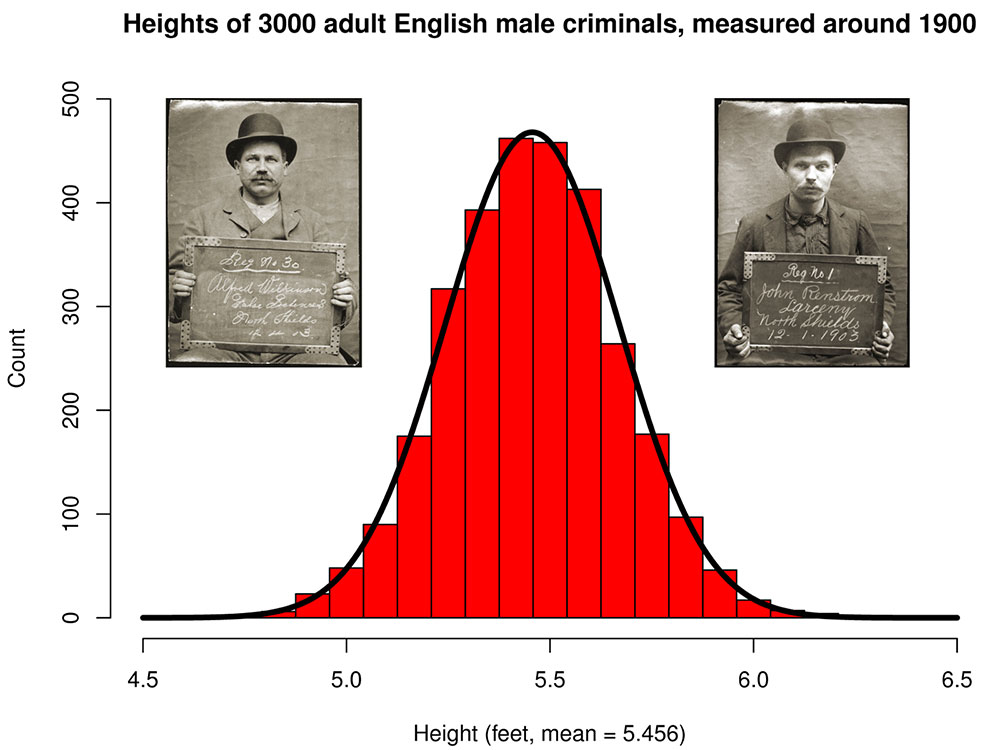
\includegraphics[width=3.10417in,height=\textheight]{heightofcriminal.jpg}

}

\caption{Kuva: A. H. Dekker.}

\end{figure}

\hypertarget{sattuman-rooli-tieteenteossa}{%
\section{Sattuman rooli
tieteenteossa}\label{sattuman-rooli-tieteenteossa}}

Sattuma vaikuttaa tieteessä monin eri tavoin, eikä sen vaikutusta voida
koskaan sulkea täysin pois.

Hyvin suunitellussa ja luotettavia menetelmiä käyttävässä
tutkimuksessakin voidaan sattuman vuoksi saada tuloksia, jotka ovatkin
vääriä.

Täten sattuman ja satunnaisuuden rooli tiivistyy erityisesti
tieteenteossa ja tieteellisten tutkimusten lukemisessa: yksi, vaikka
merkittäväkin, tutkimustulos ei ole vielä tae luotettavuudesta.

Tieteessä muistamme onneksi luottaa vain pitkän ajan saatossa
kumuloituvaan, eri tavoin koeteltuun ja tutkittuun tietoon! Erityisen
tärkeää tieteen popularisoinnissa!



\end{document}
